\chapter{Foundations of Statistical Physics}\label{sec:sm}
Statistical physics emerged in the second half of the nineteenth
century as an answer to unresolved questions in thermodynamics, the
study of heat and work. Was heat continuous and wavelike, or might it
be something else, discrete and atomic? Founding figures in the field,
including Rudolf Clausius, Ludwig Boltzmann, and James Clerk Maxwell,
answered the latter. Introducing the kinetic theory of gases, these
scientists posited gases as large collections of tiny molecules and
heat flow as the net effect of unbalanced molecular collisions. These
ideas, atomic theory, were not uncontroversial. To defend these
claims, their key task would be to translate such microscopic
descriptions to experimentally-verifiable predictions~\cite{domb}.

To complicate matters, these scientists lacked equipment that could
resolve the proposed microscopic length scales, and a square cubic
centimeter of gas can contain upwards of a million million million
molecules~\cite{domb}. The key insight in statistical physics is to
focus on the properties of the collection rather than on the
individual components-- on averages and distributions rather than
microscopic details. This translating between microscopic and
macroscopic is the essence of statistical physics, and it is to this
task we dedicate our efforts.

Our investigation begins by defining a \textit{microstate}, $\bs$: a
full description of the microscopic \textit{degrees of freedom} of our
system, $\bs\eqcolon\{s_i\}$, where $s_i$ is the $i$-th DOF, some
fundamental way in which the system can vary.\footnote{For example,
  \textit{spin}, which we will encounter in the next section.} Our
aim, as statistical physicists, is to predict the outcomes of
macroscopic measurements. A key assumption of statistical mechanics is
that we can express measurement outcomes as averages over all
microstates, $\mcS$ \sref{sec:measurements-as-averages}. If we are
interested in measuring energy, $E$, our \textit{expectation}
$\expect{E}$, will be:%
\begin{equation}%
  \expect{E}\eqcolon\sum_{\bs\in\mcS} P(\bs) E(\bs)\label{eq:expectation-as-average}
\end{equation}%
Making macroscopic predictions boils down to evaluating probabilities
of microstates and sums thereof. In the following section, we will
derive the probability distribution $P(\bs)$ and encounter the first
of the fundamental challenges in statistical physics. We follow the
treatment of Domb~\cite{domb} and Cardy~\cite{cardy}.

\section{Probabilities and Partition Functions}
Let us consider an example: we begin with some physical system,
$\mcS$. It could be metal or really anything. As we previewed, the
microscopic details will not matter to the macroscopic picture. To
measure macroscopic properties of $\mcS$, we need its distribution
over microstates $\bs$, $P(\bs)$. The trick is to introduce a
\textit{reservoir}, $\mcR$, that surrounds $\mcS$. Just like
$\mcS$, the reservoir could be anything: a gas, liquid, etc. We impose
several conditions: $\mcS$ and $\mcR$ exchange only energy and the
combined system, $\mcX=\mcS\cup \mcR$ (the \textit{universe}) is
isolated. Then, the total energy, $E$, is conserved.  If we denote the
energy of microstates, $\bs$ and $\br=\setr$ as $E(\bs)$ and $E(\br)$, respectively, this
requires $E(\bs)+E(\br)=E$.\footnote{Let us consider how $\bs$ and
  $\br$ might exchange energy physically. If $\bs$ is a metal and
  $\br$ a gas, then the two will transfer energy whenever gas
  particles collide against the metal, exchanging energy stored in the
  metal's vibrations with the kinetic energy of moving gas
  particles.} Furthermore, we treat $\mcS$ as a much smaller fraction of
$\mcX$ than $\mcR$, though $\mcS$ is still macroscopic
($1\ll\abs{\bs}\ll\abs{\br}$, where $\abs{\bx}$ denotes the number of
degrees of freedom of $\bx$).

The fundamental assumption of statistical mechanics states that, for
an isolated system, each microstate is equally probable. Then, our
probability distribution is $P(\bx)=1/\Omega(\bx)$, where
$\Omega(\bx)$ is the number of possible microstates
$\bx$. Probabilities over subsets of such a system may be more
complicated. Consider that the probability of $\bs$ is proportional to
the number of ways we can rearrange the reservoir, keeping the energy
constant. If we let $\Omega_{\br}(\bs)$ denote the number of
microstates, $\br$, with this energy $E-E(\bs)$:
\begin{equation}%
  P(\bs)=c \Omega_{\br}(\bs),
\end{equation}%
where $c$ is the constant of proportionality. By the fundamental
assumption of statistical mechanics, the above holds for any choice in
microstate, $\bs'$:
\begin{equation}%
  P(\bs')=c \Omega_{\br}(\bs').
\end{equation}%
Although we do not have enough information to evaluate absolute
probabilities, we can now compare the relative likelihood of different
microstates.
\begin{equation}%
  \frac{P(\bs)}{P(\bs')}=\frac{\Omega_{\br}(\bs)}{\Omega_{\br}(\bs')}.\label{eq:prob-ratios}
\end{equation}%
To transform the above into a more manageable form, we introduce the
Boltzmann Entropy:%
\begin{equation}%
  S(\bS)\eqcolon k \log \Omega(\bS),\label{eq:boltzmann-entropy}
\end{equation}%
where $k$ is Boltzmann's constant, a scaling factor from the
microscopic to macroscopic. Another crucial definition is that of
\textit{macrostate}: a collection of microstates, $\bS\subset \mcS$,
indistinguishable to the experimental observer.  $\Omega(\bS)$ is the
number of microstates corresponding to a macrostate,
$\Omega(\bS)=\abs{\bS}$. We interpret $S(\bS)$ as a measure of
uncertainty: higher entropy gives a lower probability of correctly
guessing the true microstate the system occupies.

Returning to the task at hand, we can apply our equation for entropy
to the reservoir into \fref{eq:prob-ratios}. Then, we get:%
\begin{equation}%
  \frac{P(\bs)}{P(\bs')}=e^{\frac{1}{k}(S_{\br}(\bs)-S_{\br}(\bs'))}.\label{eq:boltzmann-entropy-difference}
\end{equation}%

By our assumption that the reservoir is much larger than $\mcS$, we can
approximate the above using the second law of thermodynamics,
$T \Delta S \approx \Delta E$ (constant volume and number of
particles), to get:\footnote{For other statistical ensembles, we might
  include other terms, like the number of particles.}
\begin{equation}%
  \frac{P(\bs)}{P(\bs')}=e^{-\b(E_{\bs}(\bs)-E_{\bs}(\bs'))},\label{eq:boltzmann-energy-difference}
\end{equation}%
where $\b\eqcolon 1/(kT)$, the thermodynamic beta. This requires that
$\mcS$ and $\mcR$ are in thermal equilibrium, i.e.  their temperatures
are the same (for a more thorough justification of these steps, see
\fref{sec:delta-s-delta-e}). Separating (and by the fact that $\bs$
and $\bs'$ are independent), we get that:%
\begin{equation}%
  P(\bs)\propto e^{-\b E(\bs)}.
\end{equation}%

By normalizing (solving $\sum_{\bs } P(\bs)=1$), we get an equation
for the probability distribution, having used only the fundamental
assumption of statistical mechanics.\footnote{The other approximations
  become exact in the thermodynamic limit that the number of particles
  goes to infinity, \fref{sec:delta-s-delta-e}.}. We have derived the
Boltzmann distribution:%
\begin{equation}%
  \boxed{P(\bs)\eqcolon\frac{1}{Z}e^{-\b E(\bs)}\quad Z\eqcolon\sum_{\bs} e^{-\bE(\bs)}}\label{eq:boltzmann-distribution}
\end{equation}%
where $Z$ is the normalizing factor, \textit{the partition
  function}. It holds for any system $\bs$ so long as $\bs$ exchanges
only energy with its surroundings. Together, these conditions---fixed
temperature, number of particles, and volume---form the
\textit{canonical ensemble}. We have found a relation between the
energy of a microstate and its probability. If we specify an energy
function, we can calculate probabilities and, from those
probabilities, our desired measurement outcomes. In
\fref{sec:rbm-energy}, we will see this equation show up again. With
the appropriate choice in energy function,
\fref{eq:boltzmann-distribution} characterizes certain neural
networks, and much of our subsequent analysis will translate readily.

\paragraph{Ising Model.}
An example of a system with a suitable energy function for the
Boltzmann distribution is the Ising model depicted in
\fref{fig:ising}. In this model, we require that the microscopic
degrees of freedom $s_i$ are binary-valued ($s_i \in \{1,-1\}$), and
we call these degrees of freedom, \textit{spins}. The Ising model was
conceived as a minimal model for \textit{ferromagnetism}, the
phenomenon by which metals form permanent magnets. In nature, spin is
an intrinsic property of particles that induces and interacts with
magnetic fields. Though it is a quintessentially quantum effect, we
can approximate spin classically as orienting either ``up'' or
``down'' ($+1$ and $-1$ respectively).

\begin{figure}[ht]
  \centering 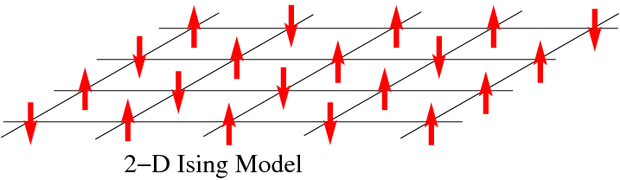
\includegraphics[width=0.5\textwidth]{figures/ising.png}
  \caption{The Ising model is a minimal model for
    ferromagnetism. Image from~\cite{ising}.\label{fig:ising} }
\end{figure}

We write the following \textit{Hamiltonian} (energy function) for the
Ising model:%
\begin{equation}
  E(\bs)\eqcolon -B \sum_i s_i-J \sum_{\langle i,j\rangle} s_i s_j,
  \label{eq:ising-energy}
\end{equation}%
where, in the ferromagnet, $B$ is the external magnetic field, $J$ is
the interaction energy between neighboring pairs of spins, and
$\sum_{\langle i, j \rangle}$ denotes a sum over adjacent sites. We
see that the system is in a lower energy state when spins $s_i$ align
with $B$ and their neighbors $J\sum_{j \rightarrow i} s_j$, where
$j\rightarrow i$ denotes the neighbors of $i$.

\paragraph{Intractable sums. } For the Ising model in one and two
dimensions, we can plug this Hamiltonian into
\fref{eq:boltzmann-distribution} and derive exact solutions for
expectation values.  Unfortunately, for the vast majority of
conceivable Hamiltonians, \fref{eq:boltzmann-distribution} is
intractable. This stems from $Z$, the \textit{partition function}.
For an Ising magnet with $N$ spins, $Z$ will contain $2^N$
terms. Beyond around $N=300$, this exceeds the number of atoms in the
universe~\cite{guth-n-atoms}. In the standard thermodynamic limit that
$N$ goes to infinity, this diverges. Even in everyday (finite) life,
$N$ is on the order of Avogadro's number, already an incredibly large
number. How are we to proceed? To complicate matters further,
\fref{eq:expectation-as-average} requires another sum of $2^n$
terms. It turns out that, with regard to this last quandary, $Z$ will
be our saving grace. $Z$, more than \textit{just} a normalizing
factor, contains all the relevant information about our system. From
$Z$, we can determine any desired macroscopic parameters of interest
by taking derivatives. For example, if we define the free energy,
$F\eqcolon-\b \ln Z$, then for the Ising model, our
expectation for the magnetization will be $\expect{M}= \partial_B F$
\sref{sec:Z-to-macros}, where $M(\bs)\eqcolon\sum_{i} s_i$, the net
orientation of all spins.

For most models of interest, then, our only option is approximation.
One class of possibilities is Markov Chain Monte Carlo (MCMC)
techniques. Rather than evaluate our sums and averages over all
microstates, $\mcS$, we evaluate these over a representative, finite
sets of samples, $\mcS_{data}$ \sref{fig:mcmc}. The trick in MCMC is
that relative probabilities, $P(\bs')/P(\bs)$, are much easier to
evaluate than absolute probabilities, $P(\bs)$, since the partition
functions cancel. Monte Carlo techniques proceed according to some
variation of:
\begin{enumerate}
\item Initialize a random state, $\bs$.
\item Consider a small variation to the state, $\bs'$ (for example, by
  flipping spin $s_i$).
\item Decide whether to accept this variation according to
  $P(\bs')/P(\bs)$.
\item Repeat steps 2 and 3 until $\bs'$ converges the
  \textit{equilibrium distribution}, $P(\bs')$.
\end{enumerate}
With modern computers, we can easily generate and average over many
samples using techniques like the Metropolis-Hastings algorithm or
cluster methods like the Swendsen-Wang and Wolff
algorithms.\footnote{For more, see, for example~\cite{mcmc}
  and~\cite{cluster-mcmc}} Crucially, computers cannot simulate
infinite lattices, and the behavior of finite lattices will differ
considerably from the infinite limit.\footnote{Any finite sum of
  analytic terms is finite, so in nature, there are no true
  divergences or critical points
  \sref{sec:crit-phenomena}. Fortunately, we can correct for these
  effects with finite-size scaling theory, a consequence of RG
  \sref{sec:finite-size-scaling}.} It was not until relatively
recently (on the timeline of statistical physics) that we could
generate appropriately large sample sizes. For these reasons, among
others, physicists devised a number of other strategies. The first we
will consider is mean-field theory (MFT).
\begin{figure}[ht]
  \centering 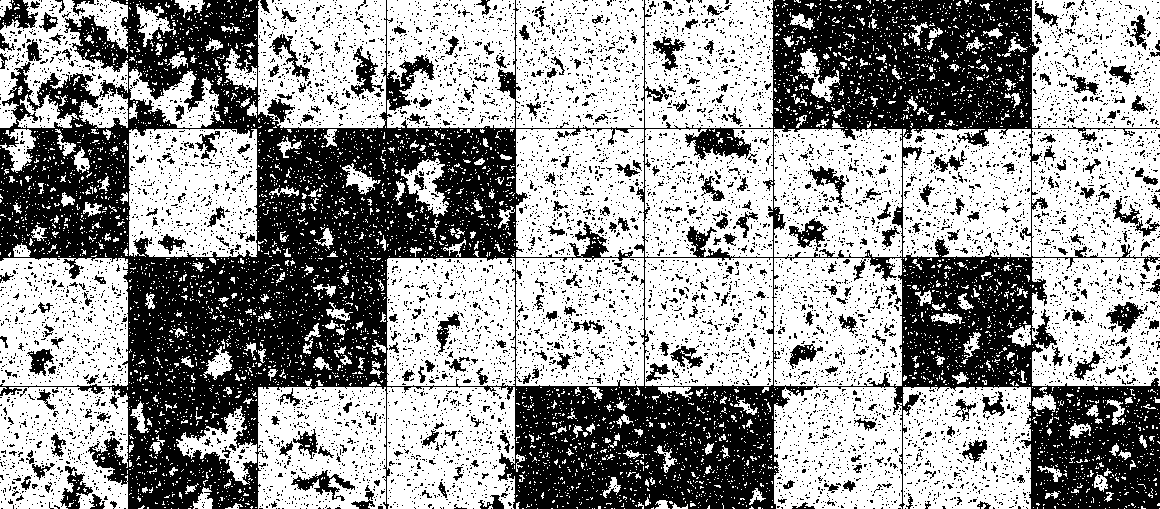
\includegraphics[width=\textwidth]{figures/samples.png}
  \caption{Samples of the 2D Ising model near the critical temperature
    generated with the Swendsen-Wang Algorithm, implemented
    \textit{rgpy}.\label{fig:mcmc} }
\end{figure}

\section{Mean-Field Theory}
To start, let us consider a simpler problem. Given a single spin
$s_i$, and a specification of all other spins, can we calculate its
partition function? We can rewrite \fref{eq:ising-energy} more
instructively:%
\begin{equation}%
  E(\bs)=-\sum_i E_i(s_i),\tab E_i(s_i)\eqcolon-\left(\sum_{j\rightarrow i} J s_j + B\right)s_i= -(nJ\expect{s_{j\rightarrow i}}+B)s_i,
\end{equation}%
where $n$ is the number of neighbors of $s_i$ and
$\expect{s_{j\rightarrow i}}\eqcolon\frac{1}{n}\sum_{j\rightarrow i} s_j$ is the average
spin of $s_i$'s neighbors. Then, the probability over $s_i$ is:
\begin{equation}%
  P(s_i)=\frac{e^{-\b (nJ\expect{s_{j\rightarrow i}}+B)s_i}}{e^{-\b (nJ\expect{s_{j\rightarrow i}}+B)}+e^{\b (nJ\expect{s_{j\rightarrow i}}+B)}},
\end{equation}%
and
\begin{equation}%
  \expect{s_i}=P(s_i=1)-P(s_i=-1)= \frac{2\cosh \b (nJ\expect{s_{j\rightarrow i}}+B)}{2\sinh \b (nJ \expect{s_{j\rightarrow i}}+B)}=\tanh \b (nJ\expect{s_{j\rightarrow i}}+B).
\end{equation}%
The orientation of a given spin depends on the average orientation of
its neighbors, as one might expect.

If we were given $\expect{s_{j\rightarrow i}}$, this sum is
trivial. Just as it is easy to calculate relative probabilities, it is
easy to calculate conditional probabilities like
$P(s_i\rvert \{s_{j\rightarrow i}\})$. Here too, the partition
functions cancel:
$P(s_i\rvert \{s_{j\rightarrow i}\})=P(s_i,\{s_{j\rightarrow i}\})/
P(\{s_{j\rightarrow i}\})$.\footnote{This avoiding of joint
  probabilities with clever choices in conditional probabilities will
  be the basis for efficiently training RBMs in the next section.}

For now, though, these observations are not of much help since we do
not know $\expect{s_{j\rightarrow i}}$. This brings us to the
mean-field approximation. Since we could have chosen any spin $s_i$ as
our starting point (including its neighbors), we expect,
$\expect{s_i}\approx\expect{s_{j\rightarrow i}}$. This is the
\textit{principle of mediocrity}. In the mean-field approximation, we
assume, more stringently that, $\expect{s}\eqcolon\expect{s_i}=\expect{s_{j\rightarrow i}}$, so:
\begin{equation}%
  \expect{s}=\tanh (\b n J \expect{s}+B).\label{eq:transcendental}
\end{equation}%
If we find a solution, then, using
$\expect{M(\bs)}=\expect{\sum_i s_i}=\sum_i \expect{s_i}$, we would
have our measurement outcome:%
\begin{equation}%
  \expect{M(\bs)}=\sum_i \expect{s_i}= N \expect{s},
\end{equation}%
and we see that $\expect{s}$ is nothing more than
magnetization per site $m=\expect{M}/N$.

It turns out that we cannot solve \fref{eq:transcendental}
analytically (it is a transcendental equation), so we have to resort
to numerical techniques. For intuition though, we can get far with a
graphical approach \sref{fig:mft}.
\begin{figure}[ht]
  \centering 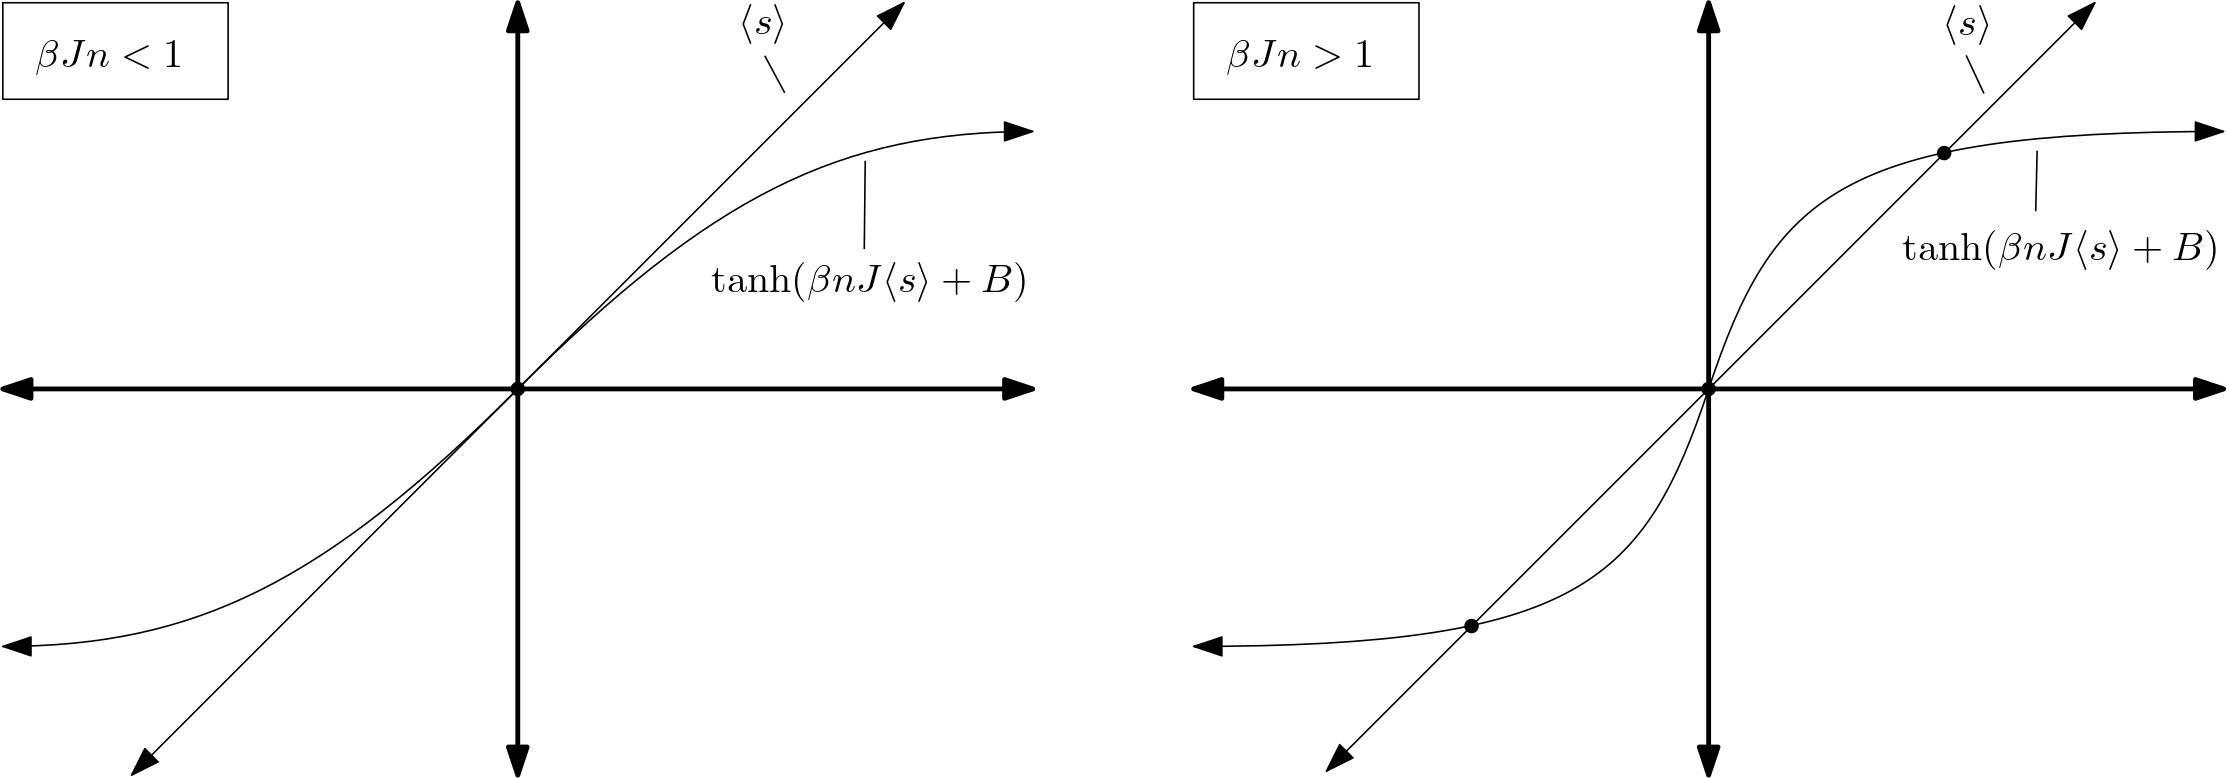
\includegraphics[width=\textwidth]{figures/mft.png}
  \caption{Mean-Field Theory predictions for the spontaneous
    magnetization $M\rvert_{B=0}$.\label{fig:mft} }
\end{figure}

Restricting to the case that $B=0$, let us distinguish two cases:
\begin{enumerate}
\item $\b J n < 1$. There is only one solution: $m=0$.
\item $\b J n > 1$.  Suddenly, there are two additional
  solutions. Something interesting seems to happen at the point
  $\b J n =1$; we call this a \textit{critical point}, and it occurs
  at the \textit{critical temperature}, $T_c= J n / k$.
\end{enumerate}

Taylor-expanding the right side of \fref{eq:transcendental}, we get
that, in the vicinity of the critical point:%
\begin{equation}%
  m
  \begin{cases}
    =0 & T>T_c\\
    \sim \pm {(3\abs{t})}^{-1/2} & T<T_c,
  \end{cases}\label{eq:mft-magnetization}
\end{equation}%
where $t$ is the \textit{reduced temperature}, $t\eqcolon(T-T_c)/T_c$.
In fact, these equations contain more information about our system
than the magnetization alone. We can use mean-field theory to derive
other parameters like the magnetic susceptibility and specific heat
(see \fref{tab:macroparameters}, some are particular to Ising-like
models, others are more general). Furthermore, our discussion assumed
an arbitrary number of neighbors, $n$, so we would expect this to hold
for any number of dimensions. It seems we have accomplished our goal
for this chapter a full section in advance.
%
\begin{center}\label{tab:macroparameters}
  \begin{table}
  \caption{Macroscopic Parameters of the Ising model}
  \begin{tabular}{ll}
    \toprule
    Macroparameter & Description\\
    \midrule
    Magnetization, $M\eqcolon\sum_i s_i$. & The strength of the magnet's field.\\
    Spontaneous magnetization, $M\rvert_{B\rightarrow 0}$ & Magnetization even\\
    &in the absence of an external magnetic field.\\
    Zero-field susceptibility, $\chi \eqcolon\partial_B M$ & How much the \\
    &magnetization changes for small changes in temperature.\\
    Energy, $\expect{E}$ & The average energy of our system.\\
    Specific heat, $C\eqcolon\partial_T \expect{E}$ & How much the average \\
    &energy changes for small changes in temperature.\\
    Correlation length, $\xi$ & The average distance across which spins are \\
    &correlated.\\
    \bottomrule
  \end{tabular}
  \end{table}
\end{center}
%
Unfortunately, in less than four dimensions, mean-field theory
provides incorrect predictions: \fref{eq:mft-magnetization} is
wrong. Intuitively, systems with less than four dimensions have too
little order for MFT to hold. More dimensions mean more paths between
any two spins and more correlation between them. Past the
\textit{critical dimension} of four, there is enough order for our MFT
approximation to hold. We have to resort to a different approach.

\section{Critical Phenomena and the Renormalization
  Group}\label{sec:crit-phenomena}
Although the quantitative predictions of the mean-field theory are
incorrect, its qualitative predictions are instructive and its
predictions about the existence of a critical point particularly
so. From \fref{eq:mft-magnetization}, we expect a phase transition
between a paramagnetic, disordered phase, and a ferromagnetic, ordered
phase (in which the system spontaneously magnetizes). This bears out
experimentally though not at the predicted temperature, see
\fref{fig:crit-exponents}.

\begin{figure}[ht]
  \centering
  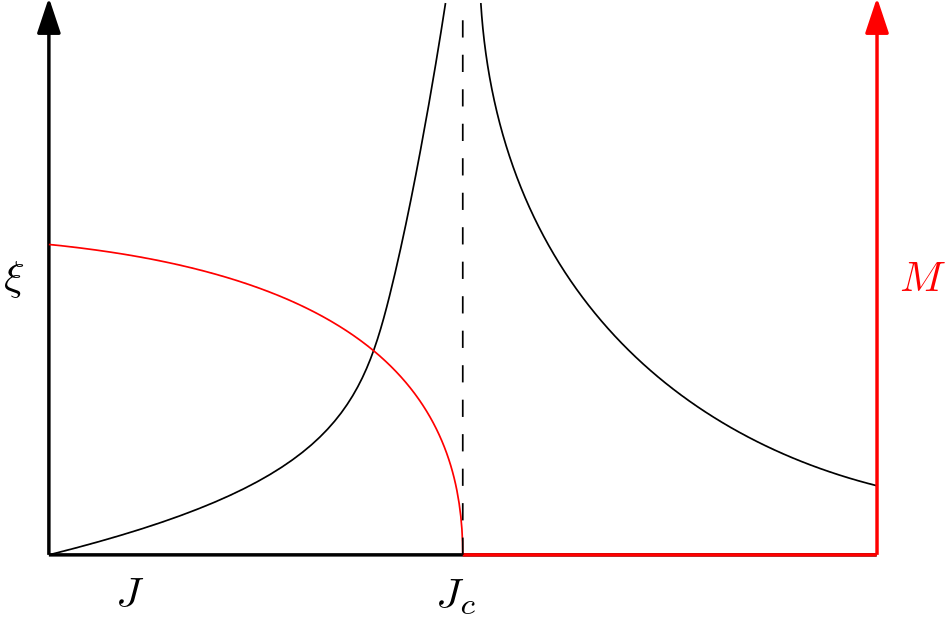
\includegraphics[width=.5\textwidth]{figures/correlation-length.png}
  \caption{The qualitative behavior of the correlation length, $\xi$,
    and magnetization, $M$, around the critical
    point.\label{fig:crit-exponents} }
\end{figure}

\paragraph{Correlation Length.} An important quantity in
\fref{tab:macroparameters} is the correlation length, $\xi$. This is
the average distance across which spins in our lattice tend to
fluctuate together. Spins farther apart than $\xi$ are effectively
independent of one another, so severing such a connection has no
appreciable effect on the macroscopic properties: we can think of
$\xi$ as a measure of how macroscopic our system
is~\cite{cardy}. Mean-field theory predicts that, near the critical
point, the correlation length scales as:%
\begin{equation}%
  \boxed{\xi\sim \abs{t}^{-1/2}}\label{eq:mft-correlation-length}
\end{equation}%

Although the exponent does not line up with experimental results (the
true value is $1$), mean-field theory correctly predicts that $\xi$
diverges at the critical point \sref{fig:crit-exponents}. In fact,
this is the defining characteristic of critical points. When the
correlation length diverges the entire system becomes correlated. Any
perturbation, no matter how infinitesimal, will have macroscopic
ramifications. For the statistical physicist, critical points are
excellent places to test theories as they allow closer access to the
microscopic realm.

\paragraph{Critical Exponents.} Another valuable prediction of
mean-field theory is that of \textit{critical exponents}. We see from
\fref{eq:mft-correlation-length} and \fref{eq:mft-magnetization} that,
near the critical point, the correlation length and the magnetization
obey simple power-laws. These are examples of a more general trend:
near critical points, macroparameters will follow power-law scaling
formulas. We call the exponents that define these relations
\textit{critical exponents} \sref{tab:crit-exponents}

\begin{table}
  \begin{center}\label{tab:crit-exponents}
    \caption{Critical Exponents of the Ising Model.}
  \begin{tabular}{lll}
    \toprule
    Critical Exponent & Macroparameter & Power Law\\
    \midrule
    $\alpha$ & Specific heat $C$ & $C\sim A \abs{t}^{-\alpha}$\\
    $\beta$ & Spontaneous magnetization $M$ & $\lim_{B\rightarrow 0}M\propto \abs{t}^\b$\\
    $\gamma$ & Zero-field susceptibility $\chi$ & $\xi\equiv\partial_B M\rvert_{B=0}\propto \abs{t}^{-\gamma}$\\
    $\delta$ & Magnetization $M$ & $M \propto \abs{B}^{1/\delta}\rvert_{t=1}$\\
    $\nu$ & Correlation length, $\xi$. & $\xi\propto\abs{t}^{-\nu}$\\
    \bottomrule
  \end{tabular}
\end{center}
\end{table}

We shift our goal to the (correct) calculation of these critical
exponents. To this end, we turn to the renormalization group, a set of
ideas for tackling precisely these critical phenomena.

\paragraph{The Renormalization Group.} Instead of trying to compute
$Z$ head-on, let us consider a different angle.  We will try to
re-express $Z$ with a simpler set of parameters while preserving the
physical, long-distance information. Repeating these transformations,
we will discard more and more irrelevant, microscopic fluctuations,
keeping only the macroscopic information. Formally, an RG
transformation will look something like:
\begin{equation}%
  \sum_{\bs'}e^{-H'(\bs')}=\sum_{\bs}e^{-H(\bs)},
  \label{eq:rg-transformation-general}
\end{equation}%
constraining for example $\abs{\bs'}<\abs{\bs}$. We consider $H'$ and
$H$ parameterized with sets of couplings $\{K'\}$ and $\{K\}$, for
example,%
\begin{equation}%
  H(\bs)=-\sum_i K^{(1)}_{i} s_i - \sum_{\expect{i,j}}K^{(2)}_{ij}s_i s_j-\sum_{\expect{\expect{i,j}}}K^{(3)}_{ij}s_i s_j\ldots,
\end{equation}%
where $\expect{\expect{i,j}}$ denotes next-nearest neighbors, and the
continued sum will, in general, contain all possible interactions. For
$K^{(1)}_i=\b B$, $K^{(2)}_{ij}=\b J$, we recover the Ising
Hamiltonian.

Alone, \fref{eq:rg-transformation-general} is not enough of a
requirement. A ``good'' RG transformation satisfies a special set of
criteria: it should preserve long-distance information while
discarding short-distance information. Arbitrary transformations
satisfying \fref{eq:rg-transformation-general} need not extract the
information we deem \textit{relevant}. Formally, we are interested in
extracting the \textit{relevant operators}, those describing
macroscopic properties, and suppressing the \textit{irrelevant
  operators}, those describing microscopic properties.  For example,
we might accomplish this transformation by summing over even spins
(known as \textit{decimation}):
\begin{equation}%
  e^{-H'(\bs')}=\sum_{s_2,s_4,\ldots,s_N} e^{-H(\bs)},
\end{equation}%
where now $\bs'$ ranges over the odd spins. In other words, we
\textit{integrate out} or \textit{marginalize over} the short-distance
degrees of freedom.

\begin{figure}[ht]
  \centering
  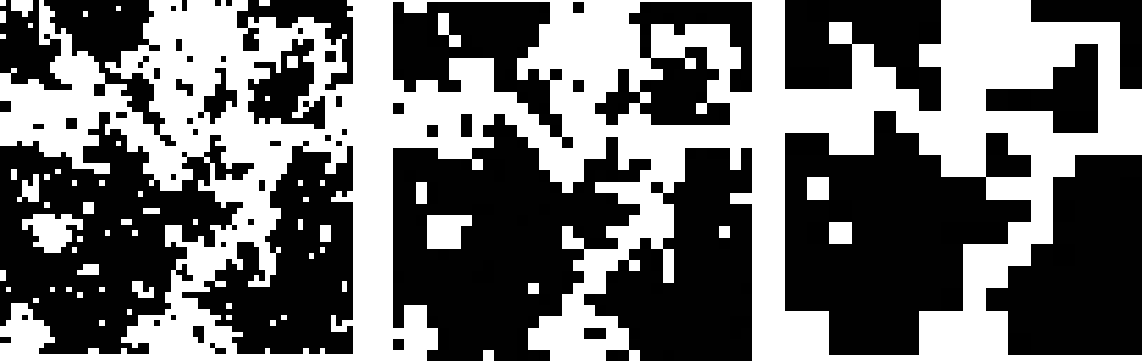
\includegraphics[width=.5\textwidth]{figures/block-rg.png}
  \caption{Three steps of majority-rule block-spin renormalization,
    preceding left to right (block size $b=2$).\label{fig:block-rg} }
\end{figure}

Consider, first, a descriptive example: (majority-rule) block-spin
renormalization, a set of RG techniques intended for lattice
systems. For a given microstate, block renormalization proceeds as
follows, \sref{fig:block-rg}:%
\begin{enumerate}
\item We partition the configuration into non-overlapping blocks. For
  each block, we determine which spin is in the majoriy, and we assign
  that value to a new, single spin. These define a new coarse-grained
  system.
\item We rescale the coarse-grained configuration so that each block
  takes the size of an original spin.
\end{enumerate}
oFormally, we can write the block transformation rule as:%
\begin{equation}%
  e^{-H'(\bs')}\eqcolon\sum_{\bs} \prod_{\text{blocks}} \pi(s'; s_i)e^{-H(\bs)},\label{eq:block-rg-transformation}
\end{equation}%
where $\pi$ is the projection operator implementing the majority rule%
\begin{equation}%
  \pi(s',s_1,\ldots,s_9)\eqcolon
  \begin{cases}
    1,&\text{if } s'=\sgn{\sum_i s_i}\\
    0& \text{otherwise.}
  \end{cases}
\end{equation}%
Though we can easily perform this procedure for any individual
configuration, \fref{eq:block-rg-transformation} requires us to do
this for all microstates, and this remains intractable. Ultimately,
for most systems, RG will use variational schemes~\cite{cardy}. It is,
however, the qualitative insights RG offers, in spite of these
approximations, which merit our immediate attention.

Consider what happens when we apply block renormalization to Ising
configurations at different temperatures as in
\fref{fig:block-rg-flow}. We see three trajectories of block
renormalization for three different initial temperatures: below the
critical point, at the critical point, and above. Our first
observation is that these transformations induce flows away from the
critical temperature. There are three fixed points ($T=0$, $T=T_c$,
and $T=\infty$) for the Ising model, and, indeed, macroscopically
these correspond to the three phases (ordered, critical, and
disordered).

\begin{figure}[ht] \centering 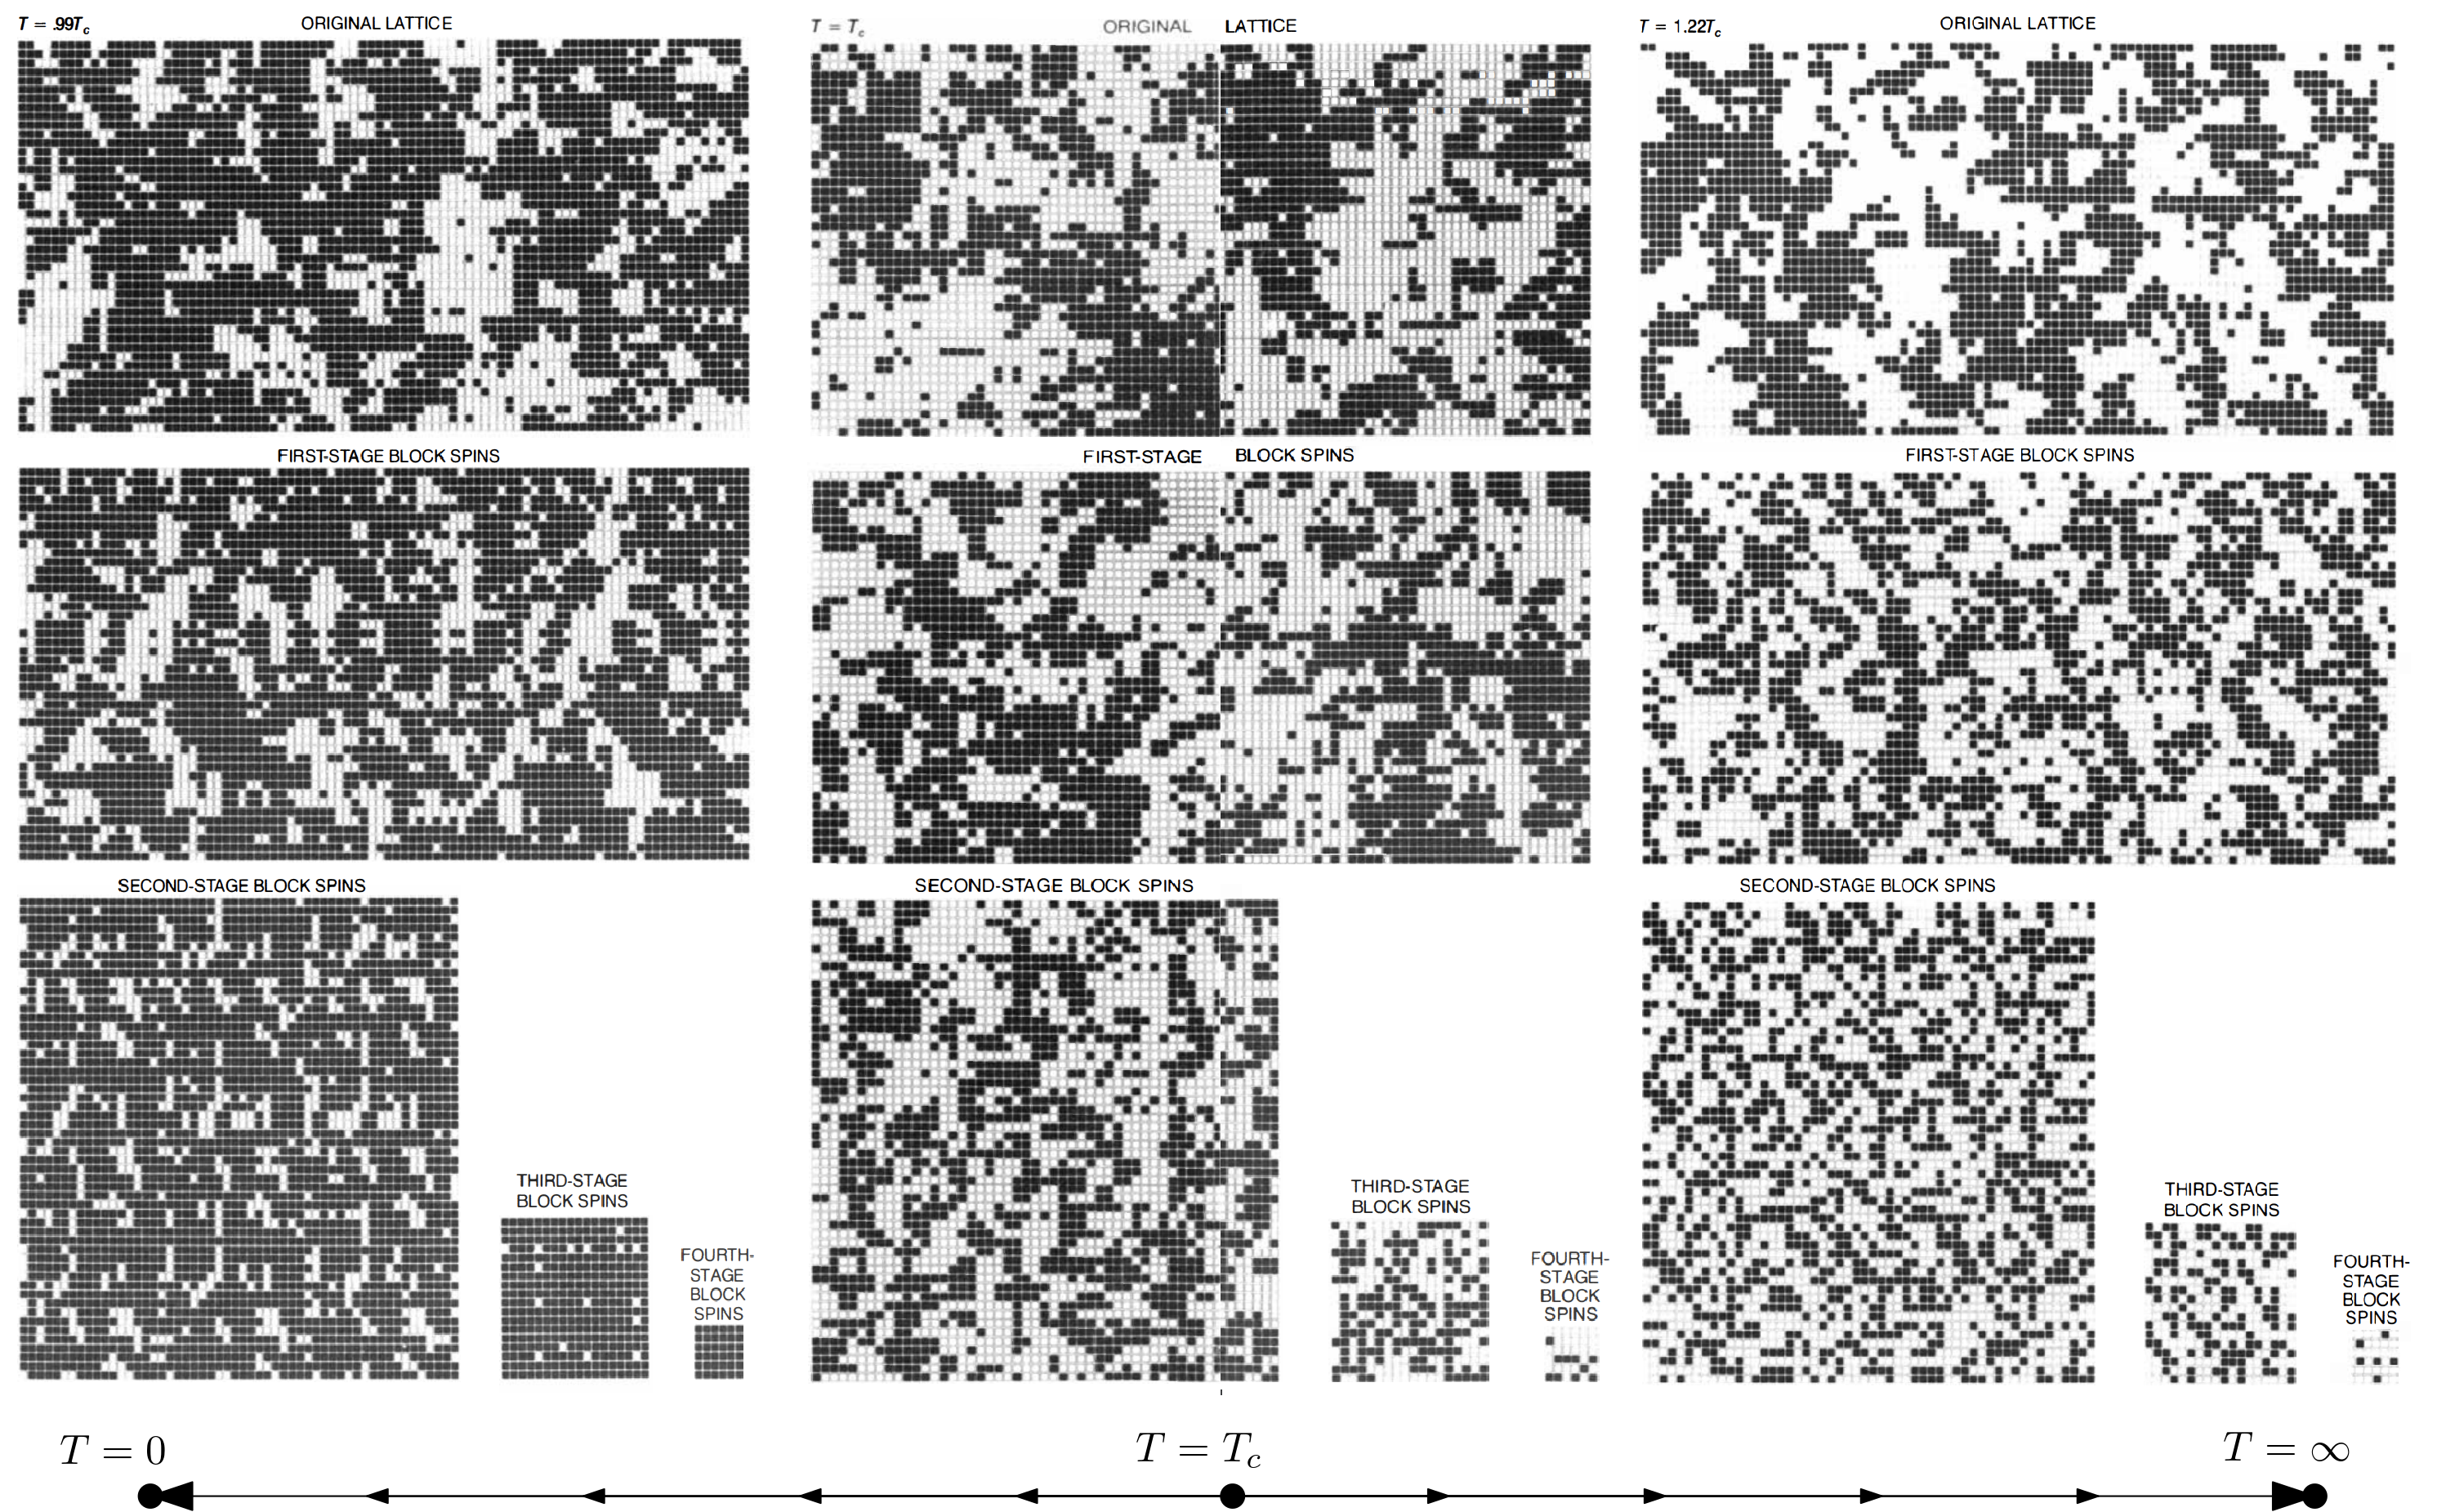
\includegraphics[
  width=\textwidth]{figures/rg-flow.png}
  \caption{Renormalization induces changes in the effective
    temperature towards fixed points. Images from
    Wilson~\cite{wilson}.\label{fig:block-rg-flow} }
\end{figure}

Let us be more exact and determine how this behavior might arise. We
will write the RG transformation rule as a function $\mc{R}$ of
couplings: $\{K'\}=\mc{R}(\{K\})$. With two general assumptions, we
can build a descriptive theory of RG\@. First, we assume that there
exists a fixed point (or multiple). These are specifications of
$\{K^*\}$ that are stable under our transformation rule, namely,
$\{K^*\}=\mc{R}(\{K^*\})$. Second, we assume we can differentiate this
transformation near the fixed point, so we can linearize:
\begin{equation}%
  K_a'\sim K_a^* + \sum_b \bolds{\mc{J}}_{ab}(K_b-K_b^*),
\end{equation}%
where $\mc{J}={\frac{\partial K_a'}{\partial
    K_b}}\rvert_{K=K^*}$. This is the Jacobian, a generalization of
the derivative to vector-valued functions of multiple variables. We
denote $\bolds{\mc{J}}$'s left eigenvectors $e^i$, corresponding to
eigenvalues, $\l^i$ so that
\begin{equation}%
  \sum_a e_a^i \bolds{\mc{J}}_{ab} = \lambda^i e_b^i.\footnote{There is no reason to assume $\bolds{\mc{J}}$ to
    be symmetric or even to have real eigenvalues though we will
    restrict ourselves to considering real-eigenvalued Jacobians.}
\end{equation}%
Next, we define \textit{scaling variables},
$u_i \eqcolon \sum_a e^i_a (K_a-K^*_a)$, which are combinations of
deviations $K_a-K_a^*$ that transform multiplicatively near the fixed
point:
\begin{align}%
  u_i'&=\sum_a e_a^i(K_a'-K_a^*)=\sum_{a,b} e_a^i \bolds{\mc{J}}_{ab}(K_b-K_b^*)\\
      &=\sum_b \lambda^i e_b^i(K_b-K_b^*)=\lambda^i u_i.
\end{align}%
For later convenience, we introduce $\l_i\equiv b^{y_i}$, where $b$ is
the rescaling size (the width of the blocks in block-spin RG). These
$y_i$ are the \textit{renormalization group eigenvalues} and are
distinguished in three cases:%
\begin{itemize}
\item $y_i>0$: $u_i$ is \textit{relevant}. Repeated RG iterations
  drive $u_i$ away from its fixed point value.
\item $y_i<0$: $u_i$ is \textit{irrelevant}. Repeated RG iterations
  drive $u_i$ towards $0$.
\item $y_i=0$: $u_i$ is \textit{marginal}. The linearized equations
  are not enough to tell us about $u_i$'s behavior.
\end{itemize}

From this, we see that our ability to distinguish between microscopic
and macroscopic is a consequence of simple dimensional analysis: there
are finitely many relevant eigenvalues. Those are the ones you see
when you zoom out far enough. The irrelevant eigenvalues span a
\textit{critical surface} of points which, under RG transformations,
are attracted towards the critical point. Macroscopically, points on
this hypersurface are indistinguishable, and their behavior is fully
characterized by the critical point alone. This brings us to the
remarkable principle known as \textit{universality}.

\paragraph{Universality.}
In the last century, experimentalists faced a puzzling situation.  In
their efforts to measure more precise critical exponents for all
manner of systems, they discovered that their experimental set-ups did
not matter: all ferromagnets for a given number of dimension possessed
the same critical exponents and so too for all
superfluids~\cite{domb}. The exponents are \textit{universal}. The
Ising model, then, is not only a minimal model for ferromagnetism, but
it can describe fluids, neural networks, metal alloys, and more.

Another key result is that we can express all of our critical
exponents in terms of the relevant RG eigenvalues. First, we use RG to
derive a scaling rule for the free energy
\sref{sec:free-energy-scaling}. Then, from its derivatives, we can
determine the critical exponents which even allows us to relate the
exponents to one another in \textit{scaling relations}. These
relations had been postulated before the advent of RG but many only as
inequalities. RG provided a rigorous means to link these different
exponents.

For example, we show a derivation in \sref{sec:rg-correlation-length}
for the correlation length critical exponent:%
\begin{equation}%
  \boxed{\nu=\frac{1}{y_t}}
\end{equation}%
where $y_t$ is the thermal RG eigenvalue, which is related, as its
name suggests, to the temperature of the system. From the exact
solution (of the Ising model in 2D), we get that $y_t=1$. Then, we
derive for the correlation length critical exponent:%
\begin{equation}%
  \boxed{\nu=1}
\end{equation}%
In general, we do not have access to solutions like these. Therefore,
we consider three approximate schemes.

\paragraph{$4-\epsilon$ Expansion.}
We can rephrase the thermodynamics limit (in which we let the number
of spins go to infinity) as the limit in which we hold the total size
of the system fixed while letting the distance between spins go to
zero. In this way, our discrete lattice becomes a continuous field,
and we can formulate the Ising model as a quantum field theory
(QFT). Whereas the above are examples of renormalization in
real-space, in QFT, we typically perform renormalization in
momentum-space. Here, we can use Wilson's $4-\epsilon$ expansion,
treating the dimensionality of our system as a
perturbation~\cite{peskin}. Then, with perturbation theory and
diagrammatics, we approximate the values of our scaling variables.

\paragraph{Monte Carlo Simulation.}\label{sec:mc-overview}
RG allows us to take advantage of the finite-size effects that
dominate Monte Carlo techniques, and we can predict how our results
will deviate from the infinite-size limits
\sref{sec:finite-size-scaling}. We can combine the two approaches,
performing the RG sums, like \fref{eq:block-rg-transformation}, over
Monte Carlo samples.\

\paragraph{Kadanoff's Variational Technique.}\label{sec:kadanoff}
Another approximation scheme is that of Kadanoff. He writes the
renormalization transformation as:
\begin{equation}%
  e^{-H'(s')}=\sum_s e^{\bT_\l(s',s)-H(s)},
\end{equation}%
where $T_\l$ a function coupling the original and coarse-grained
systems.  Kadanoff derives upper- and lower-bound estimates of the
free energy that depend on $T_\l$. By choosing $\l$ to tighten the
bounds Kadanoff variationally minimizes the difference in free energy
between the initial and coarse-grained systems, $\Delta F=F(H'~)-F(H)$
(knowing the margin of error). However, this technique does not
guarantee reasonable estimates of macroparameters.  As Kadanoff
himself observed: %

\begin{quote}
  Hopefully, one might obtain good results for physical quantities by
  choosing the upper (lower) bound recursions that give the smallest
  error in the free energy\ldots We say ``hopefully'' because usually
  one is not interested in the free energy itself. Rather its
  derivatives are of the major physical interest.  Since the
  variational principles pertain to the free energy, there is no
  guarantee that the derivatives will be accurate~\cite{kadanoff}.
\end{quote}\label{sec:kadanoff-quote}
%
This reflects one of the major challenges with RG\@.  It is by no
means ``easy'' to construct adequate RG schemes, and findings are
rarely backed with rigorous justification. The details of appropriate
transformations depend on the systems under investigation and require
an amount of intuition on the part of the physicists~\cite{kjr}.  We
will see that, ultimately, being more precise in defining
physically-relevant information will let us circumvent this problem,
formulating, a system-independent criterion of quality for RG
transformations.
